\documentclass{article}
\usepackage{graphicx}
\usepackage{listings}
\usepackage{xcolor}
\usepackage{geometry}
\usepackage{float} % Added for precise figure placement
\geometry{margin=1in}

\lstset{
    basicstyle=\ttfamily\small,
    backgroundcolor=\color{lightgray!20},
    frame=single,
    keywordstyle=\color{blue},
    commentstyle=\color{green!70!black},
    stringstyle=\color{red},
    breaklines=true,
    showstringspaces=false,
    captionpos=b,
}

\title{Brexit Election Survey Report}
\author{Pranav Jayakumar}
\date{\today}

\begin{document}

\maketitle

\section*{Introduction}
This report summarizes findings from the Brexit Election Survey dataset, with visualizations generated using Plotly Express and Python.

\section*{Python Code}
Below is the Python script used to preprocess the data and generate visualizations:

\begin{lstlisting}[language=Python, caption=Python Code for Data Analysis and Visualization]
# Visualization with Plotly Express
import pandas as pd
import plotly.express as px

# Load the dataset
df = pd.read_csv('BES2.csv')

# Add "leave_column" column
df['leave_column'] = df['vote'].apply(lambda x: True if x == 'leave' else (False if x == 'stay' else None))

# Add "age_group" column
bins = [0, 29, 60, float('inf')]
labels = ['young', 'mid-life', 'old']
df['age_group'] = pd.cut(df['age'], bins=bins, labels=labels, right=True)

# Visualization: Distribution of Age Groups
fig1 = px.histogram(df, x='age_group', title='Distribution of Age Groups', color_discrete_sequence=['#636EFA'])
fig1.write_image('age_group_distribution.png')
fig1.show()

# Visualization: Leave Votes by Age Group
fig2 = px.histogram(df, x='age_group', color='leave_column', barmode='group',
                    title='Leave Votes by Age Group', color_discrete_sequence=['#EF553B', '#00CC96'])
fig2.write_image('leave_votes_by_age_group.png')
fig2.show()

# Visualization: Leave Votes by Education Level
fig3 = px.histogram(df, x='education', color='leave_column', barmode='group',
                    title='Leave Votes by Education Level', color_discrete_sequence=['#EF553B', '#00CC96'])
fig3.write_image('leave_votes_by_education.png')
fig3.show()

print("Visualizations have been generated and saved as images.")
\end{lstlisting}

\section*{Visualizations}

\subsection*{Distribution of Age Groups}
\begin{figure}[H] % The H specifier is now controlled by the float package
    \centering
    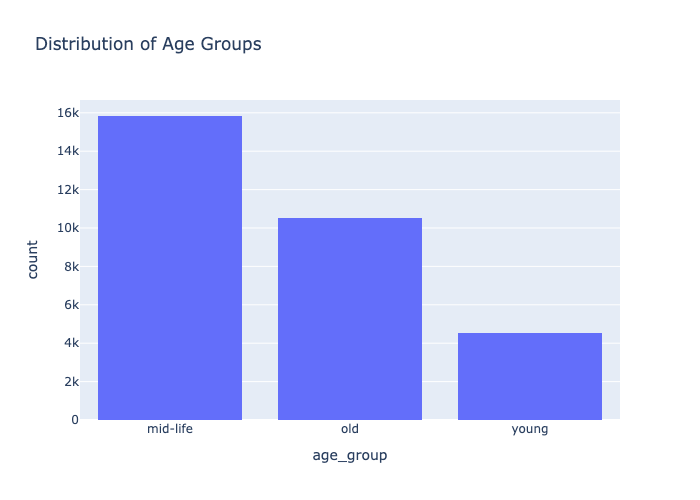
\includegraphics[width=0.8\textwidth]{age_group_distribution.png}
    \caption{Distribution of Age Groups}
\end{figure}

\subsection*{Leave Votes by Age Group}
\begin{figure}[H]
    \centering
    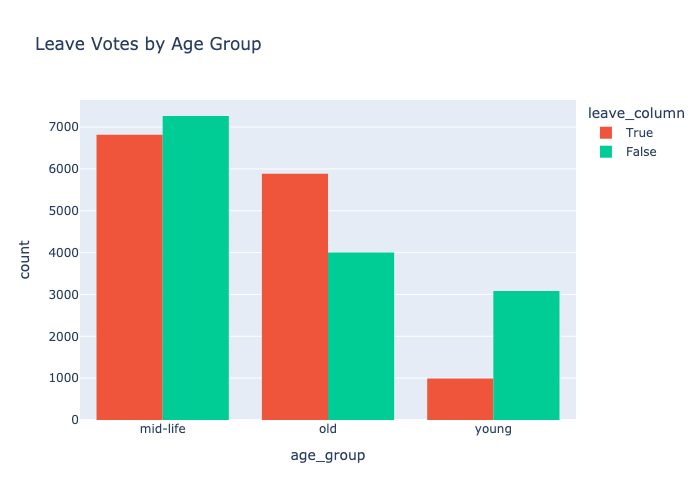
\includegraphics[width=0.8\textwidth]{leave_votes_by_age_group.png}
    \caption{Leave Votes by Age Group}
\end{figure}

\subsection*{Leave Votes by Education Level}
\begin{figure}[H]
    \centering
    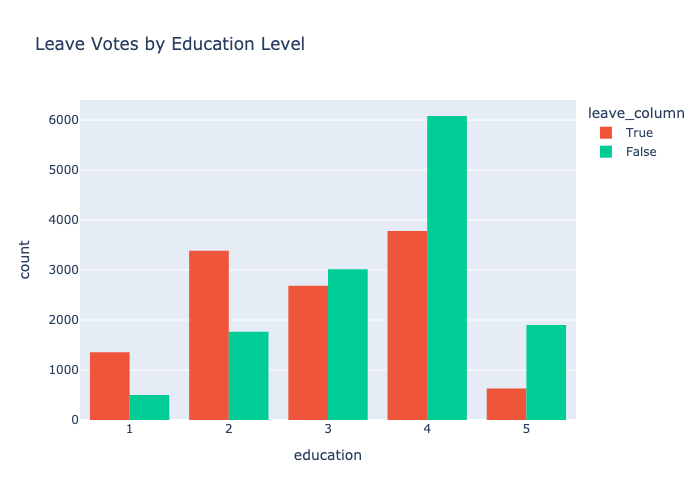
\includegraphics[width=0.8\textwidth]{leave_votes_by_education.png}
    \caption{Leave Votes by Education Level}
\end{figure}

\end{document}

